% =============================================================
\chapter{ข้อจำกัดและค่าใช้จ่าย}
\label{ch:limits}
% =============================================================

\section{ข้อจำกัดของระบบ}

\begin{enumerate}
    \item \textbf{ไม่มี HTTPS:} Learner Lab ไม่มีโดเมน จึงขอ certificate จาก ACM ให้ ALB ไม่ได้ ข้อมูลเข้าสู่ระบบส่งเป็น HTTP
    \item \textbf{WebSocket ไม่ตรวจ token:} Lambda \texttt{lorcana-room} เชื่อชื่อผู้ใช้ที่ client ส่งมา
    \item \textbf{Rate limiter อยู่ใน memory ของแต่ละ process (OWASP A07):} เมื่อมีหลาย worker และหลายเครื่อง ผู้โจมตีลองรหัสได้ 5 ครั้งคูณจำนวน worker คูณจำนวนเครื่อง แก้ได้ด้วย DynamoDB และ TTL แต่เพิ่มค่าใช้จ่ายต่อคำขอ
    \item \textbf{Secret ของ Lambda เป็น environment variable แบบ plaintext:} (EC2 อ่านจาก SSM SecureString)
    \item \textbf{เวลากู้คืน 2.8 ถึง 3.9 นาที:} ขึ้นกับเวลาบูตเครื่องใหม่
    \item \textbf{Alarm มาช้ากว่าเหตุการณ์ 2 ถึง 3 นาที:} metric ของ CloudWatch มาถึงช้า
    \item \textbf{ผลการแข่งขันรายงานจาก client:} ตัวขับเคลื่อนกฎทำงานในเบราว์เซอร์ ยังไม่มี authoritative game server ตรวจสถานะเกม
    \item \textbf{ElastiCache เป็น Node เดี่ยว:} เป็น single point of failure ของชั้นแคช (ระบบ fallback ไป DynamoDB)
    \item \textbf{CloudFront และ ElastiCache Serverless ใช้ไม่ได้:} นโยบาย IAM ของ Learner Lab ปฏิเสธ
    \item \textbf{Ability ที่ระบบจัดการอัตโนมัติเต็มรูปแบบมี 16.16\%:} ที่เหลือแสดงป้ายให้ผู้เล่นจัดการเอง
    \item \textbf{Session ของ Learner Lab ประมาณ 4 ชั่วโมง:} เครื่องถูกหยุดเมื่อหมด session
    \item \textbf{ค่าใช้จ่ายเมื่อเปิดต่อเนื่อง 24 ชั่วโมง:} ดูหัวข้อ \ref{sec:cost}
\end{enumerate}

\section{ประมาณการค่าใช้จ่าย}
\label{sec:cost}

ราคาต่อหน่วยเป็นราคา on-demand ของ us-east-1 \todo{ตรวจราคาทุกแถวกับหน้า AWS Pricing แล้วใส่วันที่เข้าถึงจริง รายงาน Phase 3 ระบุ "ตรวจสอบ 29 กันยายน 2569" แต่ Pricing API ถูกบล็อกใน Learner Lab จึงยังไม่มีการตรวจ}

\begin{table}[H]
\centering
\caption{ประมาณการค่าใช้จ่ายรายชั่วโมงเมื่อเปิด stack เต็มรูปแบบ}
\label{tab:cost_hourly}
\begin{tabularx}{\textwidth}{lXrr}
\toprule
\textbf{บริการ} & \textbf{ราคาต่อหน่วย} & \textbf{จำนวน} & \textbf{ต่อชม. (USD)} \\
\midrule
EC2 t3.micro & \$0.0104/ชม. & 2 & 0.0208 \\
EBS gp3 root 8 GiB & \$0.08/GB-เดือน & 2 $\times$ 8 GiB & 0.0018 \\
Public IPv4 & \$0.005/ชม. & 4 (EC2 2 และ ALB 2 AZ) & 0.0200 \\
ALB & \$0.0225/ชม. บวก LCU & 1 (1 LCU) & 0.0305 \\
ElastiCache t3.micro & \$0.0170/ชม. & 1 node & 0.0170 \\
Detailed monitoring & \$2.10/เครื่อง-เดือน & 2 & 0.0058 \\
CloudWatch alarm & \$0.10/alarm-เดือน & 3 & 0.0004 \\
SNS, SQS, Lambda, DynamoDB & ระดับทดสอบ & -- & $\approx$ 0.0000 \\
\midrule
\textbf{รวม} & & & \textbf{$\approx$ 0.096} \\
\bottomrule
\end{tabularx}
\end{table}

\begin{table}[H]
\centering
\caption{ค่าใช้จ่ายจริงจาก AWS Billing (1--27 กันยายน 2569)}
\label{tab:billing}
\begin{tabularx}{\textwidth}{lrr}
\toprule
\textbf{บริการ} & \textbf{ก.ย. 2569 (USD)} & \textbf{สัดส่วน} \\
\midrule
Elastic Load Balancing & 7.13 & 69\% \\
Amazon VPC (public IPv4) & 1.96 & 19\% \\
CloudWatch & 0.45 & 4\% \\
EC2 Compute & 0.44 & 4\% \\
EC2 Other (EBS) & 0.31 & 3\% \\
\midrule
\textbf{รวมตั้งแต่ต้นเดือน} & \textbf{10.29} & \\
\bottomrule
\end{tabularx}
\end{table}

ALB คิดเงินรายชั่วโมงตลอดเวลาที่ยังไม่ลบ แม้ EC2 จะถูกลดเหลือ 0 (\texttt{lab\_stop.ps1}) แล้ว ค่า Compute จึงหยุดได้ แต่ค่า ALB, Public IPv4 ของ ALB และ ElastiCache ไม่หยุด หากหยุดทดสอบเกิน 1 วัน ควรสั่ง \texttt{lab.ps1 destroy} ข้อสังเกตนี้แทนข้อความ "Scale-to-Zero ทำให้ค่าใช้จ่ายเป็น \$0.00 ต่อชั่วโมง" ในรายงานระยะที่ 2 ซึ่งใช้ได้กับค่า EC2 เท่านั้น

\subsection{ยอดค่าใช้จ่ายทั้งเดือนกันยายน 2569}

หน้า Billing and Cost Management เมื่อวันที่ 5 ตุลาคม 2569 (รูปที่ \ref{fig:billing}) แสดงค่าใช้จ่ายรวมของเดือนกันยายนทั้งเดือน 13.49 ดอลลาร์ ซึ่งสูงกว่ายอด 10.29 ดอลลาร์ในตารางที่ \ref{tab:billing} ที่นับถึงวันที่ 27 กันยายน ส่วนต่าง 3.20 ดอลลาร์เป็นค่าใช้จ่ายของวันที่ 28 ถึง 30 กันยายน ค่า CloudWatch เดือนกันยายนในภาพคือ 0.69 ดอลลาร์ และกลุ่ม Others 12.79 ดอลลาร์ ภาพนี้ไม่แยกกลุ่ม Others เป็นรายบริการ ตารางที่ \ref{tab:billing_full} จึงใช้ข้อมูลจาก AWS Cost Explorer API (\texttt{aws ce get-cost-and-usage}) ที่ดึงเมื่อวันที่ 5 ตุลาคม 2569 โดยกรองเฉพาะรายการประเภท Usage

\begin{figure}[H]
\centering
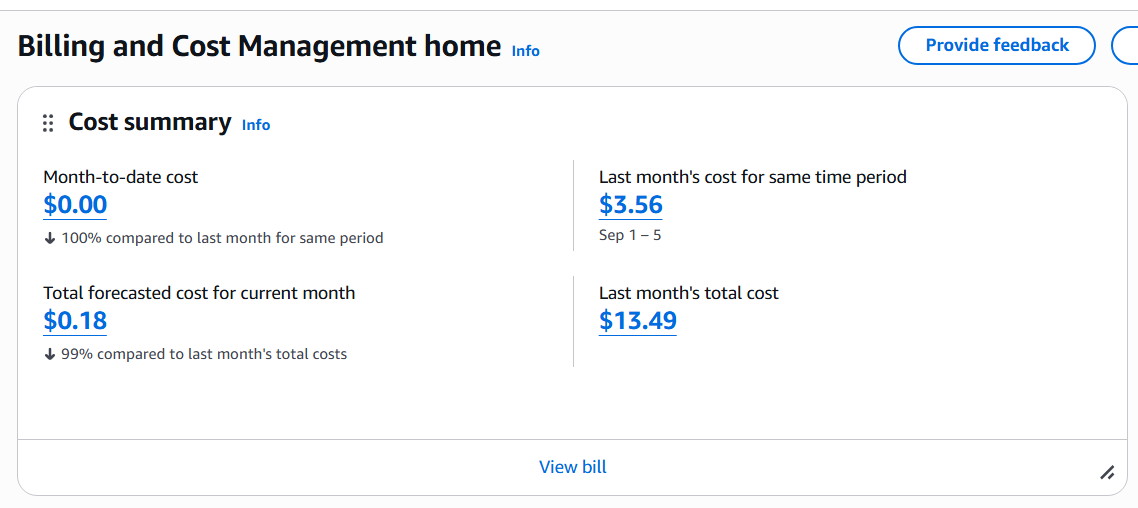
\includegraphics[width=0.78\textwidth]{images/useindoc/billing_cost_summary_2026-10-05.png}\\[0.3cm]
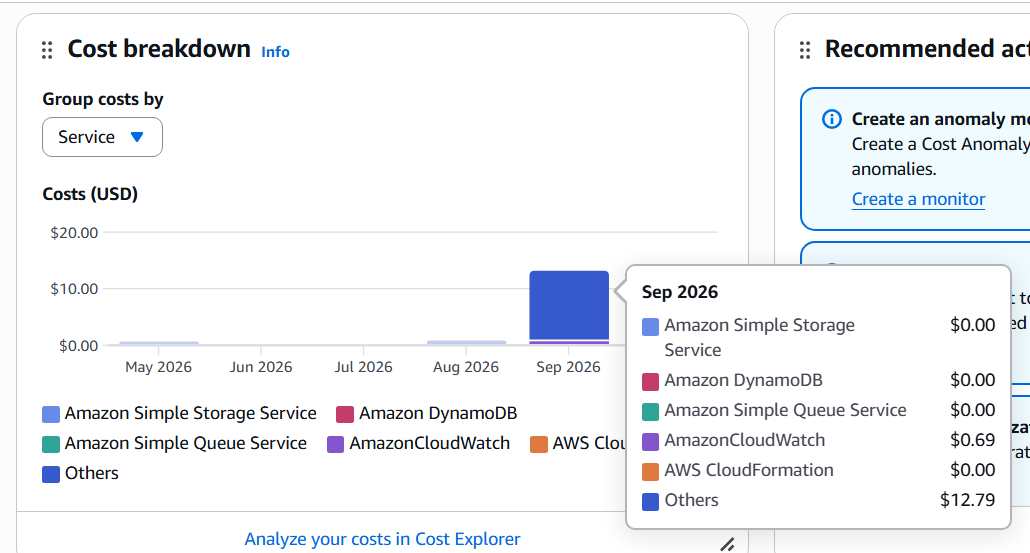
\includegraphics[width=0.78\textwidth]{images/useindoc/billing_cost_breakdown_2026-10-05.png}
\caption{หน้า Billing and Cost Management (5 ตุลาคม 2569): ยอดเดือนกันยายน 13.49 ดอลลาร์ และสัดส่วนตามบริการ}
\label{fig:billing}
\end{figure}

ค่าใช้จ่ายเดือนตุลาคมที่แสดงเป็น 0.00 ดอลลาร์ในภาพเป็นเพราะข้อมูล Billing ล่าช้ากว่าการใช้งานจริง stack ที่ deploy เมื่อวันที่ 5 ตุลาคม ยังไม่ปรากฏในยอดนี้

\begin{table}[H]
\centering
\caption{ค่าใช้จ่ายการใช้งาน (Usage) เดือนกันยายน 2569 ทั้งเดือน แยกตามบริการ (Cost Explorer API)}
\label{tab:billing_full}
\begin{tabularx}{\textwidth}{lrr}
\toprule
\textbf{บริการ} & \textbf{USD} & \textbf{สัดส่วน} \\
\midrule
Elastic Load Balancing & 7.72 & 57.3\% \\
Amazon VPC (public IPv4) & 2.36 & 17.5\% \\
EC2-Other (EBS, NAT Gateway ฯลฯ) & 1.18 & 8.8\% \\
EC2 Compute & 0.94 & 6.9\% \\
CloudWatch & 0.69 & 5.1\% \\
Amazon RDS & 0.50 & 3.7\% \\
ElastiCache & 0.07 & 0.5\% \\
AWS Cost Explorer & 0.02 & 0.1\% \\
S3, DynamoDB, API Gateway, KMS, EventBridge & 0.01 & 0.1\% \\
\midrule
\textbf{รวมค่าใช้งาน} & \textbf{13.49} & \\
เครดิตของบัญชี (Credit) & $-$13.49 & \\
\textbf{ยอดสุทธิ} & \textbf{0.00} & \\
\bottomrule
\end{tabularx}
\end{table}

ข้อสังเกตจากตารางที่ \ref{tab:billing_full}:
\begin{itemize}
    \item ค่า Elastic Load Balancing เกือบทั้งหมด (7.72 จาก 7.72 ดอลลาร์) เป็น \texttt{LoadBalancerUsage} หรือค่าชั่วโมงที่ ALB เปิดอยู่ ส่วนค่า LCU ตามปริมาณทราฟฟิกมีเพียง 0.006 ดอลลาร์
    \item ค่าใช้จ่ายรวมของเดือนสิงหาคมคือ 0.82 ดอลลาร์ และของวันที่ 1--5 ตุลาคมคือ 0.0002 ดอลลาร์ (ข้อมูลล่าช้า) รวมตั้งแต่ 1 สิงหาคมถึง 5 ตุลาคมประมาณ 14.31 ดอลลาร์ก่อนหักเครดิต
    \item ตัวเลขสุทธิเป็น 0 เพราะรายการ Credit หักค่าใช้งานทั้งหมด หน้า Billing Console แสดงยอดก่อนหักเครดิต (13.49) ส่วนรายงานจาก Cost Explorer ที่ไม่กรองประเภทรายการ และผลของ Amazon Q ที่ตอบเกือบ 0 ดอลลาร์ แสดงยอดสุทธิหลังหักเครดิต
    \item \textbf{ค่า EC2-Other มี NAT Gateway ประมาณ 13 ชั่วโมง (0.585 ดอลลาร์ ที่อัตรา 0.045 ดอลลาร์ต่อชั่วโมง) และข้อมูลผ่าน NAT อีก 0.19 ดอลลาร์ และมีค่า Amazon RDS 0.50 ดอลลาร์} สคริปต์ของโครงงานไม่สร้างทั้งสองอย่าง และขณะตรวจเมื่อวันที่ 5 ตุลาคม 2569 ไม่มี NAT Gateway หรือ RDS instance อยู่ในบัญชี AWS CloudTrail บันทึกว่าทั้งสองอย่างถูกสร้างเมื่อวันที่ 28 กันยายน 2569 เวลา 01:37 น. (NAT Gateway) และ 01:38 น. (RDS) โดย IAM user เดียวกับที่ใช้ deploy โครงงาน ห่างกัน 1 นาที ไม่ได้มาจากสคริปต์ของโครงงาน \todo{ระบุว่า NAT Gateway และ RDS ที่สร้างเมื่อ 28 ก.ย. 01:37 น. เป็นของงานอะไร (เช่น lab อื่นหรือการลองใน Console) เพื่อเขียนว่าเป็นค่าใช้จ่ายนอกโครงงาน}
\end{itemize}
